% @Author: Your name
% @Date:   2024-04-20 21:21:00
% @Last Modified by:   Your name
% @Last Modified time: 2024-04-25 10:44:42
% sectionis/method.tex

\section{Hierarchical Ensemble Framework for Co-clustering Large Matrices}
\label{sec:method}

\subsection{Overview}

In this paper, we propose a novel hierarchical ensemble framework for co-clustering large matrices as shown in \Cref{fig:workflow}. 
This contribution arises from the central idea of our method, which consists in decomposing the large matrices into smaller, digestible submatrices. Such partitioning is not arbitrary but guided to some extent by our developed optimal big matrix partitioning algorithm. It follows a probabilistic model that offers accurate estimations of the optimal number and the sequence of partitions for efficiency and effectiveness processes. Further, an important aspect is that to split the computational heavy task of co-clustering the large matrix into smaller, parallelizable tasks. This way, we will be able to sharply reduce the computational burden and achieve better scalability by our method.

Upon partitioning, co-clustering is performed to each submatrix, that is, through the application of SVD and $k$-means on the resulting singular vectors. This step is important, ensuring adaptivity in clustering; hence, the capability to adapt to the peculiar characteristics of each sub-matrix. It becomes even more flexible in the sense that this does not define the co-clustering algorithm. In our paper, we demonstrate the process with SVD and $k$-means, but any can be used meeting a certain level of accuracy.

Our approach is a novel hierarchy ensemble method that fuses cohesively and in an intelligent way the co-clustering results from all submatrices. They add, therefore, not only granularity in the insights that could be got from each of the submatrices but contribute to the overall accuracy and reliability even of the total co-clustering outcome. Our method, validated and optimized through a rigorous process, showed an efficiency in the handling of large-scale datasets that was never reached before in the history of the method. It is a significant stride in the effectiveness of methods applied to contemporary data analyses.

% insert workflow.png here
\begin{figure*}[htbp]
    \centering
    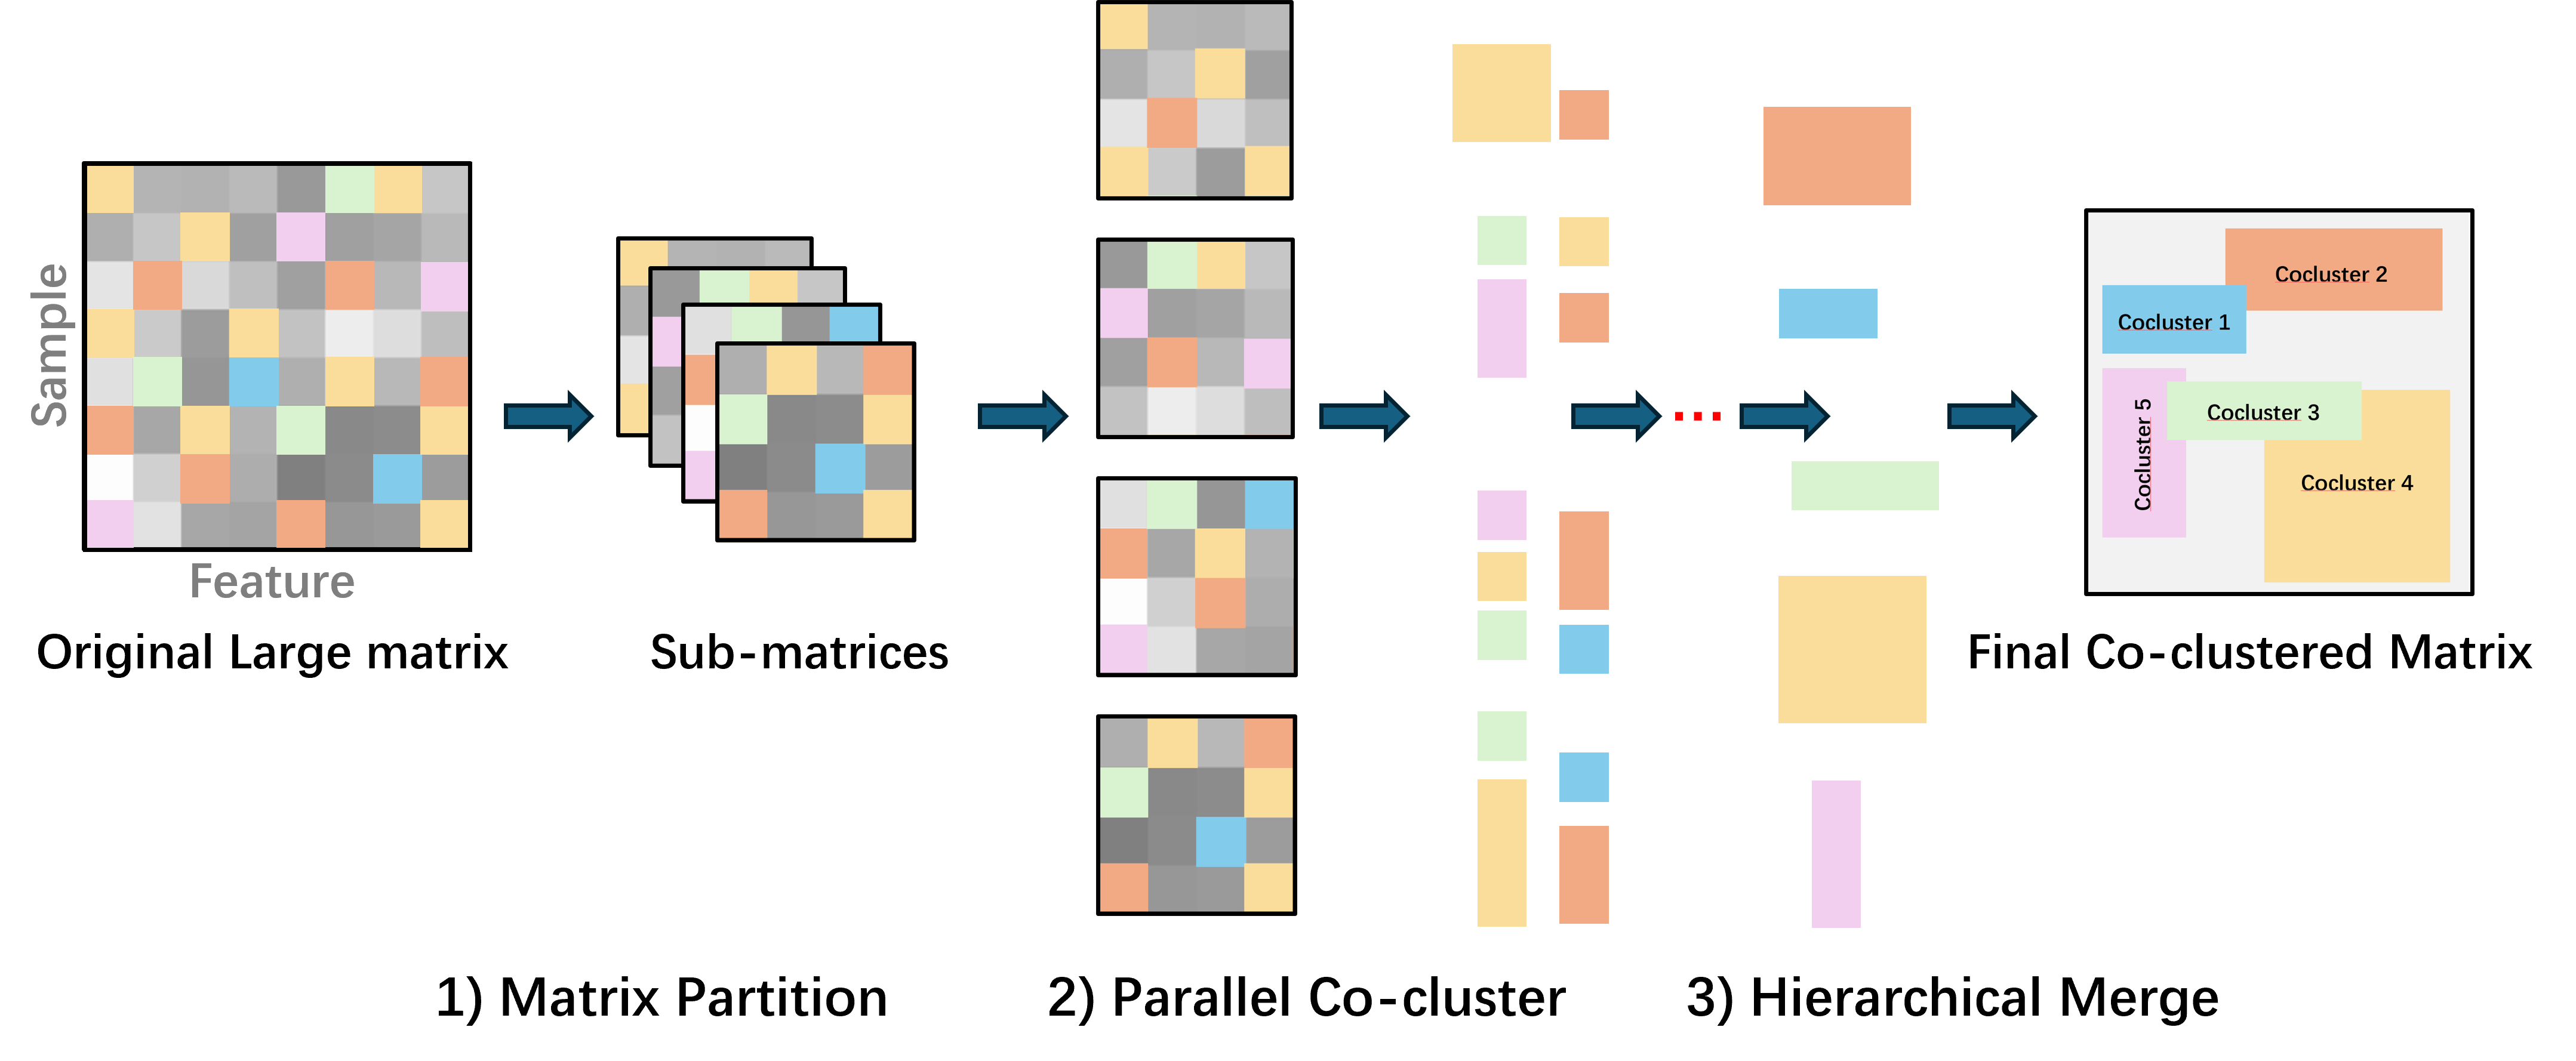
\includegraphics[width=0.8\linewidth]{workflow.png}
    \caption{Workflow of the proposed hierarchical ensemble framework for co-clustering large matrices.}
    \label{fig:workflow}
\end{figure*}

% \subsection{Notation and Definitions}
% % Definitions of symbols, notations, and terminologies used in the method.
% In this section, we define the notation and mathematical formulations used in our method. Understanding these definitions is crucial for comprehending the subsequent descriptions of the algorithm and its implementation.

% \begin{itemize}
%     \item $A \in \mathbb{R}^{M \times N}$ is a matrix with $K$ co-clusters (co-cluster set $C = \{C_k\}_{k=1}^K$);
%     \item $A$ is partitioned into $m \times n$ blocks, each block having a size of $\phi_i \times \psi_j$, implying that $M=\sum_{i=1}^m \phi_i$ and $N=\sum_{j=1}^n \psi_j$;
%     \item The block set is denoted as $B = \{B_{(i,j)}\}_{i=1}^m,_{j=1}^n$;
%     \item The size of co-cluster $C_k \in \mathbb{R}^{M^{(k)} \times N^{(k)}}$ within block $B_{(i,j)}$ is represented as $M_{(i,j)}^{(k)} \times N_{(i,j)}^{(k)}$;
%     \item $T_m$ represents the minimum number of rows, while $T_n$ denotes the minimum number of columns in a co-cluster.
% \end{itemize}

% With these notations established, we can now proceed to detail the algorithm and its components in the subsequent sections

\subsection{Problem Formulation}
The task at hand involves the analysis of a data matrix, denoted as $\mathbf{A} \in \mathbb{R}^{M \times N}$, comprising $M$ rows (representing features or variables) and $N$ columns (representing objects or samples). The entry at the $(i, j)$-th position of $\mathbf{A}$ is given by $a_{ij}$.
%, where $a_{i,\cdot}$ and $a_{\cdot,j}$ represent the $i$-th row and $j$-th column of $\mathbf{A}$, respectively

A co-cluster within this context is identified as a subset of rows and/or columns that exhibit similar characteristics across a subset of columns and/or rows. Let $I$ be a set of row indices forming a row cluster, and $J$ be a set of column indices forming a column cluster; then the sub-matrix $\mathbf{A}_{I,J}$ corresponds to a co-cluster in $\mathbf{A}$. The objective of co-clustering is to partition the $M$ rows into $k$ row clusters and the $N$ columns into $d$ column clusters, resulting in a total of $k \times d$ co-clusters.
Notably, with proper reordering of rows and columns, the co-clustered matrix $\mathbf{A}$ can be represented as a block-diagonal matrix.
With this definition, data matrix $\mathbf{A}$ can be partitioned into submatrices where the data within each submatrix is more similar to each other than to the rest of the data.

% These partitions can be represented by a row label vector $u\in\mathbb{N}^M$ (where $u_i \in \{1, \ldots, k\}, \forall i \in \{1, \ldots, M\}$) and a column label vector $v \in \mathbb{N}^N$ (where $v_j \in \{1, \ldots, d\}, \forall j \in \{1, \ldots, N\}$). Indicator matrices $R \in \mathbb{R}^{M \times k}$ (where $\sum_{k'=1}^{k} R_{i,k'} = 1$) and $C \in \mathbb{R}^{N \times d}$ (where $\sum_{d'=1}^{d} C_{j,d'} = 1$) denote the row and column clusters.

Let \( u \in \{1,\dots,k\}^M \) and \( v \in \{1,\dots,d\}^N \) be row and column label sets. Define indicator matrices \( R \in \mathbb{R}^{M \times k} \), \( \sum_k R_{i,k} = 1 \), and \( C \in \mathbb{R}^{N \times d} \), \( \sum_d C_{j,d} = 1 \), for row and column clusters.

We aim to identify co-clusters $\mathbf{A}_{I,J}$ in $\mathbf{A}$ that are correlated according to specific criteria. These criteria include co-clusters with constant values, constant values along rows or columns, and co-clusters with additive or multiplicative coherent values. Recognizing and categorizing these patterns in $\mathbf{A}$ forms the basis of our co-clustering approach, which is designed to effectively and efficiently identify such structures within the data.

\subsection{Dynamic Matrix Partitioning}
% Description of the matrix partitioning process and criteria for partitioning.
The primary challenge in co-clustering large matrices is the risk of losing meaningful co-cluster relationships when the matrix is partitioned into smaller submatrices. To address this, we introduce an optimal partitioning algorithm underpinned by a probabilistic model. This model is meticulously designed to navigate the complexities of partitioning, ensuring that the integrity of co-clusters is maintained even as the matrix is divided. The objective of this algorithm is twofold: to determine the optimal partitioning strategy that minimizes the risk of fragmenting significant co-clusters and to define the appropriate number of repartitioning iterations needed to achieve a desired success rate of co-cluster identification.

\subsubsection{Partitioning and Repartitioning Strategy based on the Probabilistic Model}
Our probabilistic model serves as the cornerstone of the partitioning algorithm. It evaluates potential partitioning schemes based on their ability to preserve meaningful co-cluster structures within smaller submatrices. The model operates under the premise that each atom-co-cluster (the smallest identifiable co-cluster within a submatrix) can be identified with a probability $p$. This probabilistic framework allows us to estimate the likelihood of successfully identifying all relevant co-clusters across the partitioned submatrices.

In the scenario where the matrix $A$ is partitioned into $m \times n$ blocks, each block has size $\phi_i \times \psi_j$, that is, $M=\sum_{i=1}^m \phi_i$ and $N=\sum_{j=1}^n \psi_j$, the joint probability of $M_{(i,j)}^{(k)}$ and $N_{(i,j)}^{(k)}$ are
\begin{align*}
    P(M_{(i,j)}^{(k)} & < T_m, N_{(i,j)}^{(k)} < T_n)                               \\ & = \sum_{\alpha=1}^{T_m-1} \sum_{\beta=1}^{T_n-1} P(M_{(i,j)}^{(k)} = \alpha) P(N_{(i,j)}^{(k)} = \beta) \\
    % pq[x_, y_] := Sum[p[a] * q[b], {a, 1, x-1}, {b, 1, y-1}]
                      & \le \exp[-2 (s_i^{(k)})^2 \phi_i + -2 (t_j^{(k)})^2 \psi_j]
\end{align*}
where $s_i^{(k)}$ and $t_j^{(k)}$ are the minimum row and column sizes of co-cluster $C_k$ in block $B_{(i,j)}$, the size of the co-cluster $C_k$ is $M^{(k)} \times N^{(k)}$, and $M^{(k)}$ and $N^{(k)}$ are the row and column sizes of co-cluster $C_k$, respectively. 

% the size of co-cluster $C_k \in \mathbb{R}^{M^{(k)} \times N^{(k)}}$ that falls into block $B_{(i,j)}$ is $M_{(i,j)}^{(k)} \times N_{(i,j)}^{(k)}$;

Thus, the probability of identifying all co-clusters given by

\begin{align}
    P(\omega_k) & \le \exp \left\{ -2 [\phi m (s^{(k)})^2 + \psi n (t^{(k)})^2] \right\},
\end{align}
and
\begin{align}
    P & = 1 - P(\omega_k)^{T_p}                                                                                                       \\
      & \ge 1 - \exp \left\{ -2 T_p [\phi m (s^{(k)})^2 + \psi n (t^{(k)})^2] \right\} \label{eq:prob_of_identifying_all_co_clusters}
\end{align}
where $P(\omega_k)$ is the probability of the failure of identifying co-cluster $C_k$, $T_p$ is the number of sampling times, $\phi$ and $\psi$ are the row and column block sizes, and $s^{(k)}$ and $t^{(k)}$ are the minimum row and column sizes of co-cluster $C_k$.


\Cref{eq:prob_of_identifying_all_co_clusters} is central to our algorithm for partitioning large matrices for co-clustering, providing a probabilistic model that informs and optimizes our partitioning strategy to preserve co-cluster integrity. It mathematically quantifies the likelihood of identifying all relevant co-clusters within partitioned blocks, guiding us to mitigate risks associated with partitioning that might fragment vital co-cluster relationships.

Based on \Cref{eq:prob_of_identifying_all_co_clusters}, we can establish a constraint between the repartitioning time $Tr$ and the partition solution $Part$, ensuring that the partitioning strategy adheres to a predetermined tolerance success rate, thereby minimizing the risk of co-cluster fragmentation. The constraints are discussed in appendix due to space limitations.

\subsubsection{Optimization and Computational Efficiency}
Optimizing the partitioning process for computational efficiency is paramount in both academic and industrial applications, where running time often serves as the primary bottleneck. Thanks to the flexible framework established by our probabilistic model and the constraints derived in Theorem 1, our optimization strategy can be tailored to address the most critical needs of a given context. In this case, we focus on minimizing the running time without compromising the integrity and success rate of co-cluster identification.
%TODO check the theorem number

Our approach to optimization leverages the probabilistic model to assess various partitioning configurations, balancing the trade-off between computational resource allocation and the need to adhere to theoretical success thresholds. By systematically evaluating the impact of different partitioning schemes on running time, we can identify strategies that not only meet our co-clustering success criteria but also optimize the use of computational resources.

To ensure that our optimization does not sacrifice the quality of co-cluster identification for the sake of efficiency, we introduce a secondary theorem that outlines the conditions under which optimization can be achieved without compromising the success rate of co-cluster discovery. This theorem provides a mathematical basis for optimizing the partitioning algorithm in a manner that maintains a balance between computational efficiency and the fidelity of co-cluster identification.


Under the constraint of maintaining a predetermined success rate $P$ for co-cluster identification, the optimization of the partitioning algorithm with respect to running time must satisfy the following condition:
\begin{align*}
    T_p = \text{argmin}_{T_p} \{ 
     1 &- \exp \{ -2 T_p [\phi m (s^{(k)})^2 \\
     &+ n (t^{(k)})^2] \} \ge P_{\text{thresh}} \} 
\end{align*}


This condition delineates the parameters within which the partitioning strategy can be optimized for speed without detracting from the algorithm's ability to accurately identify co-clusters. By adhering to this theorem, we ensure that our optimization efforts align with the overarching goal of preserving the integrity and effectiveness of co-cluster discovery. This balance is crucial for developing a partitioning algorithm that is not only fast and efficient but also robust and reliable across various data sets and co-clustering challenges.

\subsection{Co-clustering on Small Submatrices}
% Detailed method for co-clustering within each of the submatrices.

\subsubsection{Atom-co-clustering Algorithm}
Our framework, which encompasses both partitioning and ensembling, offers remarkable flexibility, allowing it to be compatible with a wide range of atom-co-clustering methods. For the sake of making this paper comprehensive and self-contained, we provide an introduction to the atom-co-cluster method herein. The only requirement for an atom-co-clustering method to be compatible with our framework is that it must be able to identify co-clusters under a given criterion with a probability $p$, or more relaxed conditions, has a lower bound estimate of the probability of identifying co-clusters equipped with a validation mechanism.

\subsubsection{Graph-based Spectral Co-clustering Algorithm}

Spectral co-clustering (SCC) stands as one of the most prevalent methods in the realm of co-clustering today\cite{vonluxburg2007TutorialSpectralClustering}, primarily due to its adeptness in unraveling the complexities of high-dimensional data. At its core, this method harnesses the power of spectral clustering principles, focusing on the utilization of a graph's Laplacian matrix eigenvectors for effectively partitioning data into distinct clusters. This approach is exceptionally beneficial for analyzing data that naturally forms a bipartite graph structure, including applications in text-document analysis, social network modeling, and gene expression studies.


\paragraph{Graph Construction in Co-clustering Expanded}

SCC begins with constructing a bipartite graph $G=(U,V,E)$. Here, $U$ and $V$, both as vertex sets, symbolize the sets corresponding to the rows and columns of the data matrix, respectively. The edges $E$ of this graph are assigned weights reflecting the relationships between rows and columns. Consequently, the graph's weighted adjacency matrix $W$ is defined as:

$$ W = \begin{bmatrix} 0 & A \\ A^T & 0 \end{bmatrix}, $$
where $A$ denotes the data matrix, also called adjacency matrix in the graph context.
Through this representation, the challenge of co-clustering is reformulated into a graph partitioning task, aiming to segregate the graph into distinct clusters based on the interrelations between the data matrix's rows and columns.

\paragraph{Laplacian Matrix}

The graph's Laplacian matrix $L$ is computed as $L=D-W$, with $D$ being the graph's degree matrix—a diagonal matrix whose entries equal the sum of the weights of the edges incident to each node. The Laplacian matrix plays a crucial role in identifying the graph's cluster structure. It does so by facilitating the calculation of eigenvectors associated with its smallest positive eigenvalues, which in turn, guide the partitioning of the graph into clusters.

\paragraph{Graph Partitioning and Singular Value Decomposition}
Theorem 4 in \cite{dhillon2001CoclusteringDocumentsWords} states that the eigenvector corresponding to the second smallest eigenvalue of the following eigenvalue problem gives the generalized partition vectors for the graph:

\begin{equation}
    L \mathbf{v} = \lambda D \mathbf{v}
    \label{eq:eigenvalue_problem}
\end{equation}

And according to Section 4 of \cite{dhillon2001CoclusteringDocumentsWords}, the singular value decomposition of the normalized matrix $A_n = D^{-1/2} A D^{-1/2}$
$$A_n = U \Sigma V^T$$
gives the solution to \Cref{eq:eigenvalue_problem}. To be more specific, the singular vectors corresponding to the second largest singular value of $A_n$ is the eigenvector corresponding to the second smallest eigenvalue of \Cref{eq:eigenvalue_problem}.

The above discussion is under the assumption that the graph has only one connected component. In a more general setting, $\mathbf{u_2}, \mathbf{u_3}, \ldots, \mathbf{u_{l+1}}$ and $\mathbf{v_2}, \mathbf{v_3}, \ldots, \mathbf{v_{l+1}}$ reveal the $k$-modal information of the graph, where $\mathbf{u_k}$ and $\mathbf{v_k}$ are the $k$-th left and right singular vectors of $A_n$, respectively.
And for the last step,
$$ Z = \begin{bmatrix} D_1^{-1/2} \hat{U} \\ D_2^{-1/2} \hat{V} \end{bmatrix} $$
is stacked where $\hat{U} = [\mathbf{u_2}; \mathbf{u_3}; \ldots; \mathbf{u_{l+1}}]$ and $\hat{V} = [\mathbf{v_2}; \mathbf{v_3}; \ldots; \mathbf{v_{l+1}}]$. The approximation to the graph partitioning optimization problem is then solved by applying a $k$-means algorithm to the rows of $Z$. More details can be found in \cite{dhillon2001CoclusteringDocumentsWords}.

\subsection{Hierarchical Ensemble Co-clustering}
% Explanation of how co-clustered results from submatrices are aggregated.

Hierarchical ensemble co-clustering is a novel approach that combines the results of co-clustering on submatrices to produce a final co-clustered result.
The ensemble method is designed to enhance the accuracy and robustness of the co-clustering outcome by leveraging the complementary strengths of multiple clustering algorithms. This approach is particularly effective in identifying nuanced patterns within each submatrix, which might be overlooked by a single clustering algorithm. The ensemble method is key to our method's ability to efficiently process high-dimensional data.

After partitioning, we apply an ensemble clustering method to each submatrix. This approach involves using multiple clustering algorithms in tandem, capitalizing on the strengths of each to achieve a more accurate and robust clustering result. The ensemble method is particularly effective in identifying nuanced patterns within each submatrix, which might be overlooked by a single clustering algorithm. This step is key to our method's ability to efficiently process high-dimensional data.

\subsection{Algorithmic Description}
% Step-by-step algorithmic description of the process in pseudocode.
Our proposed \textbf{Dynamic Partition and Hierarchical Ensembling Co-Clustering Method} is outlined in Algorithm \ref{alg:method}. The algorithm
is an advanced algorithm designed for efficient co-clustering of large data matrices. The algorithm begins by initializing a block set based on predetermined block sizes. For each co-cluster in the given set, the algorithm calculates specific values $s^{(k)}$ and $t^{(k)}$, which are then used to determine the probability $P(\omega_k)$ of each co-cluster. If this probability falls below a predefined threshold $P_{\text{thresh}}$, the algorithm partitions the data matrix $A$ into blocks $B$ and performs co-clustering on these blocks. This step is crucial for managing large datasets by breaking them down into smaller, more manageable units. After co-clustering, the results from each block are aggregated to form the final co-clustered result $\mathcal{C}$. The algorithm's design allows for a flexible and efficient approach to co-clustering, particularly suited to datasets with high dimensionality and complexity.

\begin{algorithm}[!t]
    \caption{Dynamic Partition and Hierarchical Ensembling Co-Clustering Method}\label{alg:method}
    \begin{algorithmic}[1]
        \REQUIRE{Data matrix $A \in \mathbb{R}^{M \times N}$, Co-cluster set $C = \{C_k\}_{k=1}^K$, Block sizes $\{\phi_i\}_{i=1}^m$, $\{\psi_j\}_{j=1}^n$, Thresholds $T_m$, $T_n$, Sampling times $T_p$, Probability threshold $P_\text{thresh}$;}
        \ENSURE{Co-clustered result $\mathcal{C}$;}
        \STATE Initialize block set $B = \{B_{(i,j)}\}_{i=1}^m,_{j=1}^n$ based on $\phi_i$ and $\psi_j$
        \STATE Calculate $s^{(k)}$ and $t^{(k)}$ for each co-cluster $C_k$
        \FOR{$k=1$ to $K$}
        \STATE Calculate $P(\omega_k)$ for co-cluster $C_k$
        \IF{$P(\omega_k) < P_{thresh}$}
        \STATE Partition matrix $A$ into blocks $B$ and perform co-clustering
        \STATE Aggregate co-clustered results from each block
        \ENDIF
        \ENDFOR
        \RETURN Aggregated co-clustered result $\mathcal{C}$
    \end{algorithmic}
\end{algorithm}